\documentclass{VRARWorkshop}

\usepackage[utf8]{inputenc}
\usepackage[T1]{fontenc}
\usepackage[hidelinks]{hyperref}

\title{Augmented reality for supporting manual non-destructive ultrasonic testing of metal pipes and plates}

% \authors{Robert Deppe, Oliver Nemitz, Jens Herder}
\authors{}

\affiliations{~}
% TODO: Correct affiliations

\abstract{
The aim of this paper is to describe the application of augmented reality technology in non–destructive testing of products of the metal–industry and a prototype created in the course of a bachelor--thesis.
The prototype is created with hard– and software, that is usually employed in the gaming industry, and delivers positions for creating c–-scans.
Using a stereocamera in combination with a HMD enables realtime visualisation of the probes path in the HMD, as well as the setting of virtual markers on the specimen.
As a part of the implementation the downhill–simplex optimization–algorithm is implemented to fit the specimen to a cloud of recorded surfacepoints.
The accuracy is statistically tested and evaluated.
This paper is of interest not only for research–-institutes of the metal–-industry, but also for any areas of work, in which the enhancement with augmented–reality is possible.
}

% Give some keywords
\keywords{
Nondestructive Testing,
Ultrasonic,
Augmented Reality,
Tracking,
Stereo--camera,
HTC,
ZED,
NDT,
AR
}

\begin{document}

\section{Introduction}

\begin{figure}[h!]
    \begin{center}
        \includegraphics[width=79mm]{images/US-workspace.jpg}
        \caption{\label{fig:europipe} Workspace for manual ultrasonic-testing of steel pipeline pipes at Europipe in Mülheim an der Ruhr.}
    \end{center}
\end{figure}

\begin{figure}[h!]
    \begin{center}
        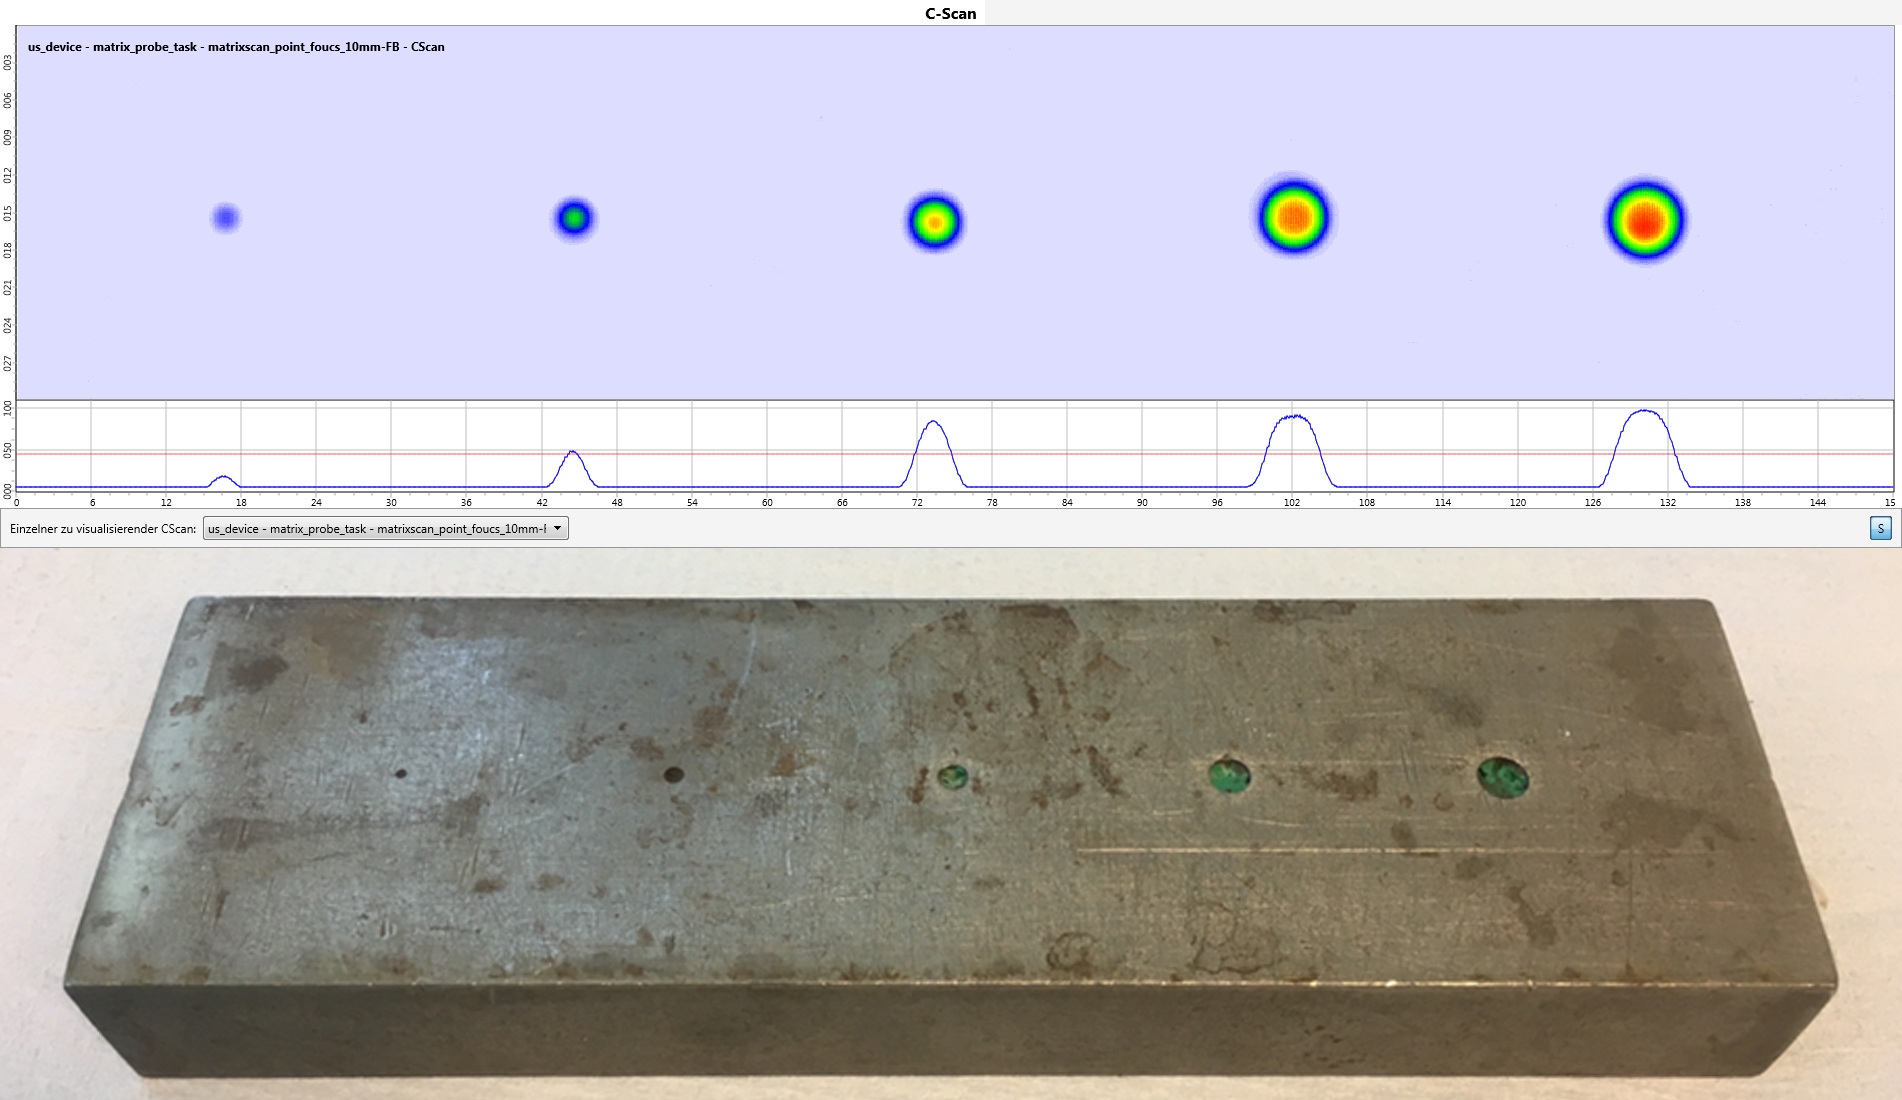
\includegraphics[width=79mm]{images/CScan.jpg}
        \caption{\label{fig:cScan} C--Scan with a resolution of 0,1\,mm}
    \end{center}
\end{figure}

\section{Related Research}
In the 2015 released patent \textit{A system and method of non-destructive inspection with a visual scanning guide} \textit{Olympus} patented the procedure of enhancing the manual inspection with AR--Glasses which help to trace a predefined inspection--plan path.
The patent describes details like tolerated deviation from the inspection path.
However there is no mentioning of the possibility to log specific points or the traced path on the probe \cite{ARPat15}.\\

The article \textit{Non-contact tracking of phased-array probe and real-time generation of C-scans for the inspection of composite aerospace structures} describes a system, which uses a stereocamera and active markers to determine the probes position and orientation on a possibly curved surface of plane components \cite{walter_non-contact_2007}.\\

A similar system, supporting the cleaning of surfaces is presented in the article \textit{Cleaning Up With Augmented Reality} by Alice Bonasio.
It describes the advantages of using AR-technology, like a DRAW or HYBRID system (section~\ref{sec:DrawVsErase}), can have on quality assurance in the commercial cleaning industry \cite{ARClean}.\\

\cite{fadzil_design_2015}\\

\section{Basics of non-destructive ultrasonic testing of metal products}
\cite{deutsch_zfp_2010}
\cite{moles_introduction_2004}
\cite{olympus_Grundlagen}

\section{Description of the AR--application}
The AR--application supports manual testing visually, and sends the aquired position data to the inspection software, which is connected via an IP connection.
Through a AR-HMD the inspector is able to see the already inspected path and identify gaps.
Position and Rotation is send to the ultrasonic scanning computer, where the data is combined with the measurements received by the probe into a C--Scan.

\section{Implementation}
The application was implemented in the game--engine Unity.
Attached to the HMD is the \textit{ZEDmini}, a stereo--camera that can be used to display a camera image in the HMD and to create a depth mask.

\cite{dorner_virtual_2013}

\begin{figure}[h!]
    \begin{center}
        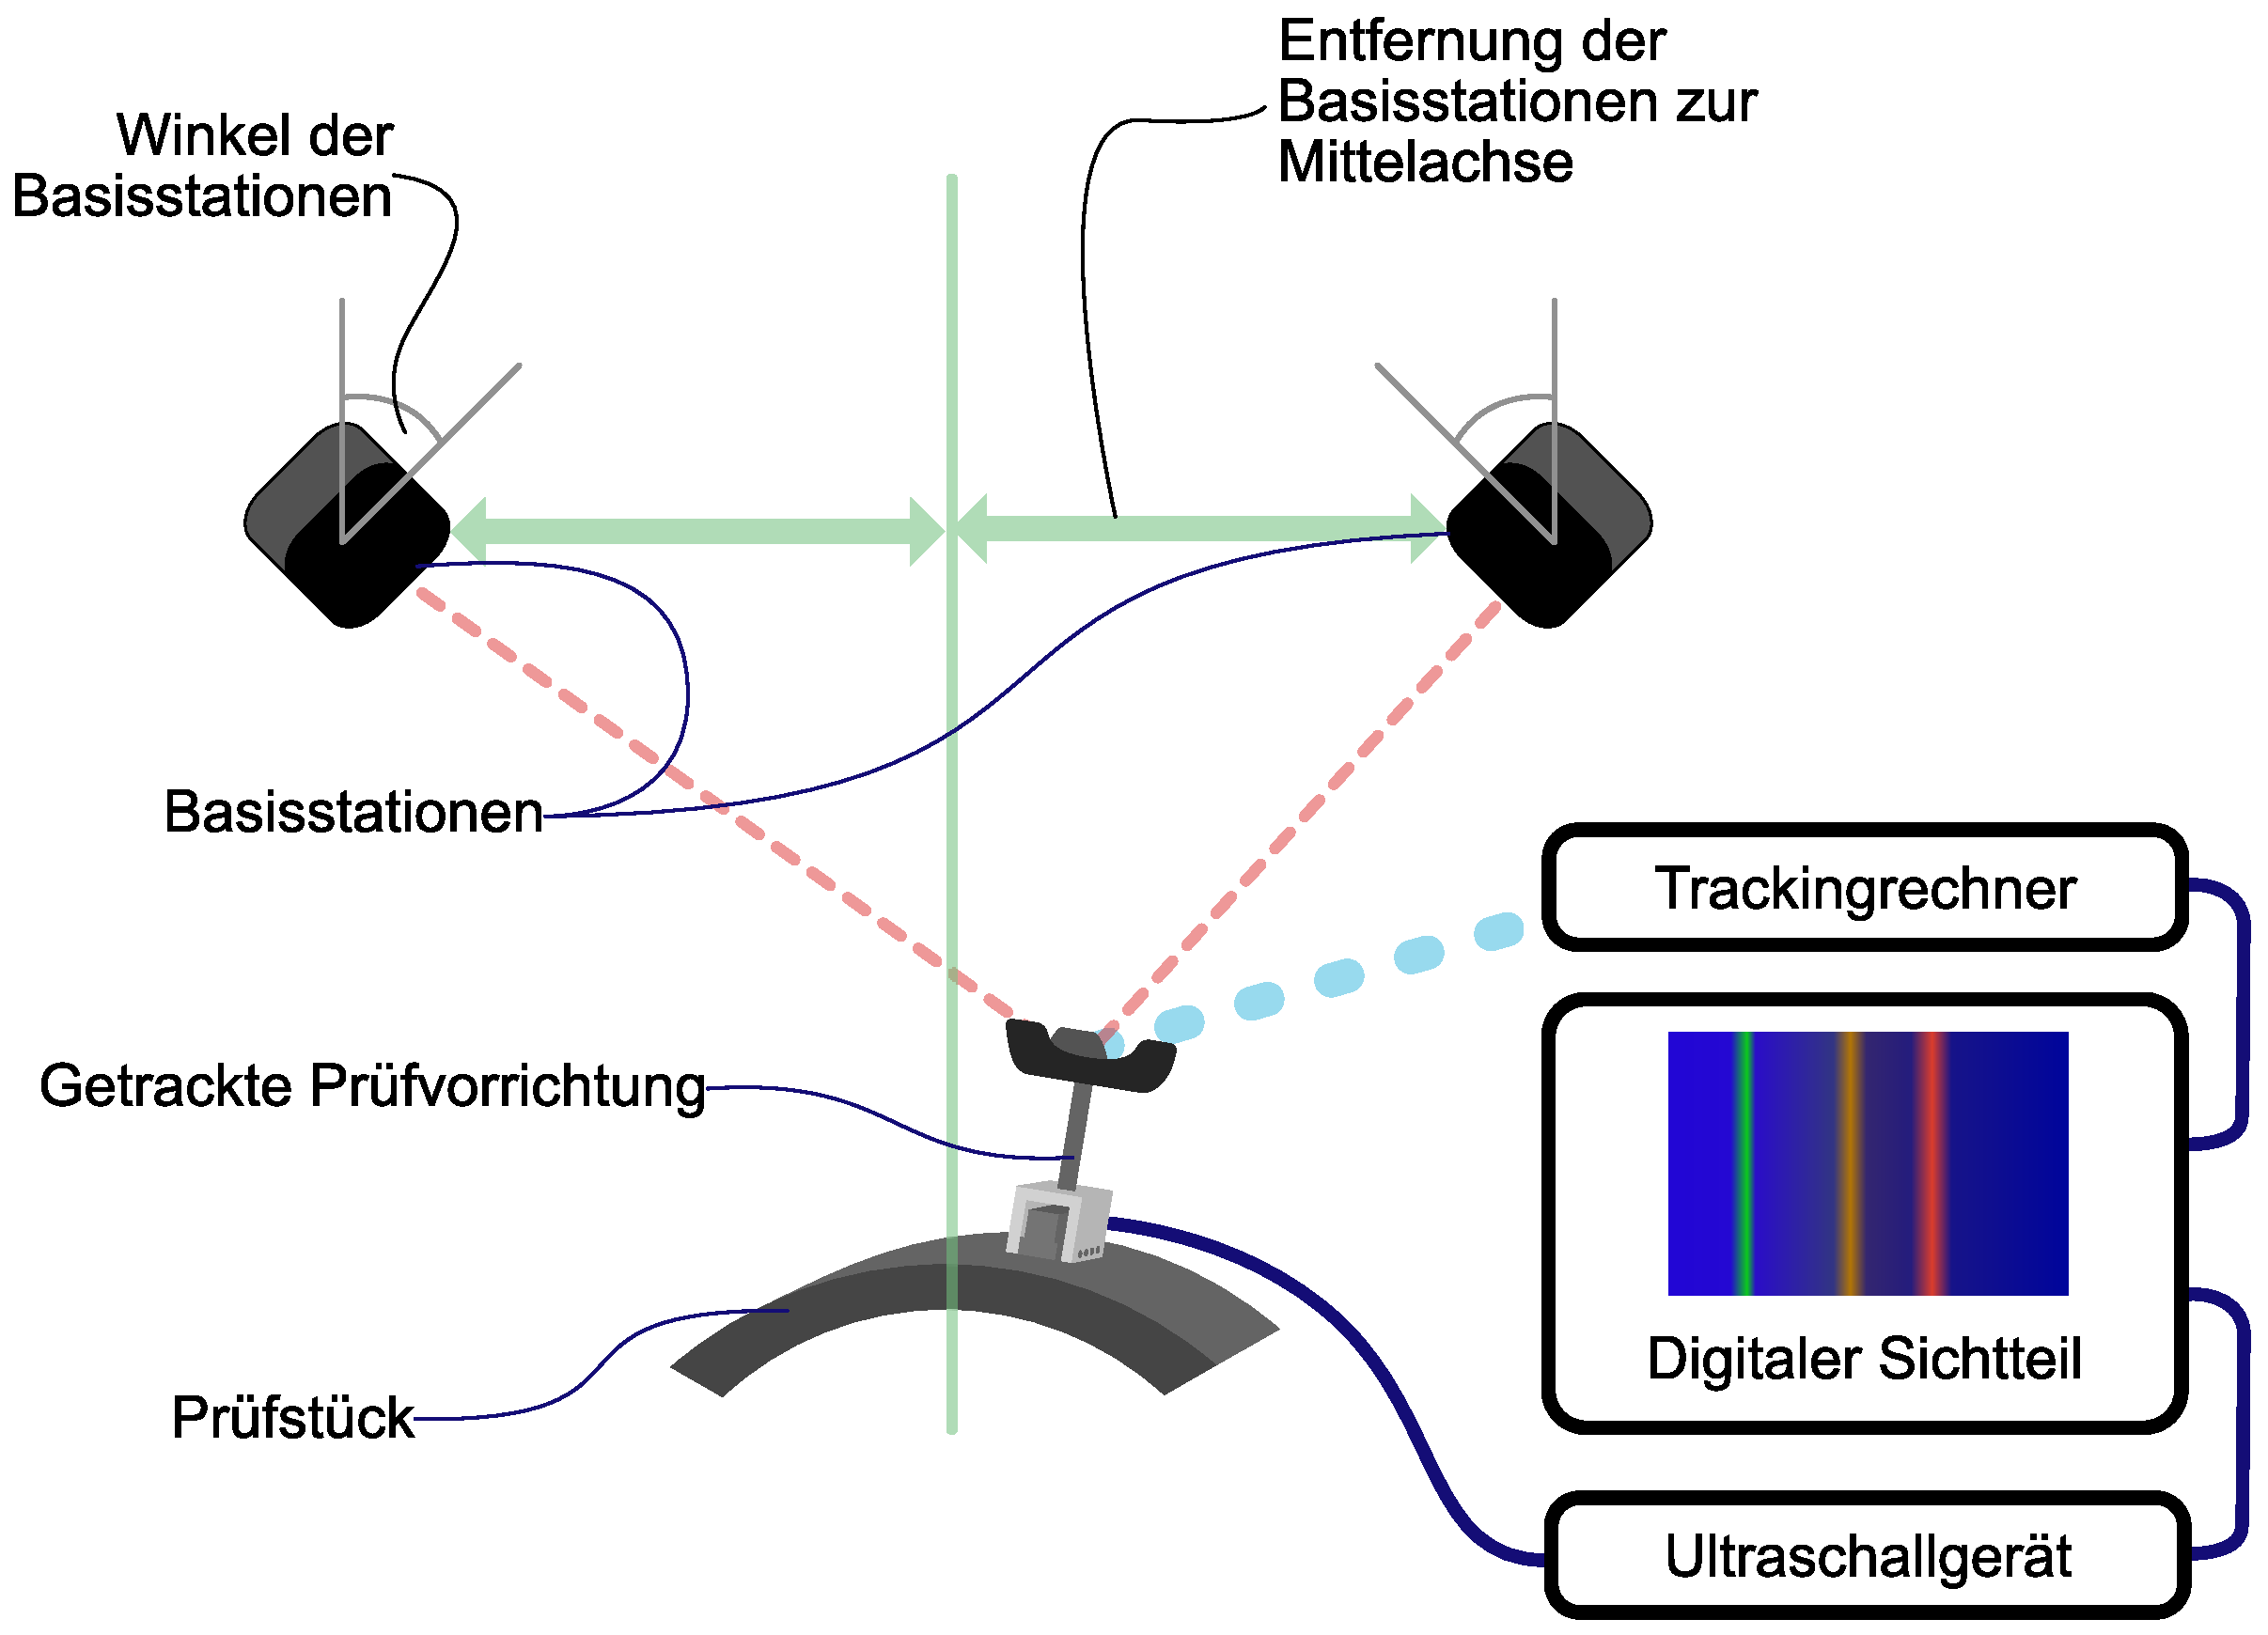
\includegraphics[width=79mm]{images/Setup.eps}
        \caption{\label{fig:Setup} Setup of the described AR-application. \textcolor{red}{Grafik muss noch übersetzt werden.}}
        % TODO: Grafik übersetzen, ZEDmini hinzufügen
    \end{center}
\end{figure}

\subsection{Tracking of the ultrasonic probe}
The ultrasonic probe is tracked with the help of a attachable tracked \textit{VIVE}--Tracker.
This Tracker is attached to a mount, in which the ultrasonic probe is fixed (figure~\ref{fig:probemount}).
The offset and orientation between the tracker and probe is applied in software by setting the virtual probe as a child transform of the tracker.

\begin{figure}[h!]
  \label{fig:probemount}
    \begin{center}
        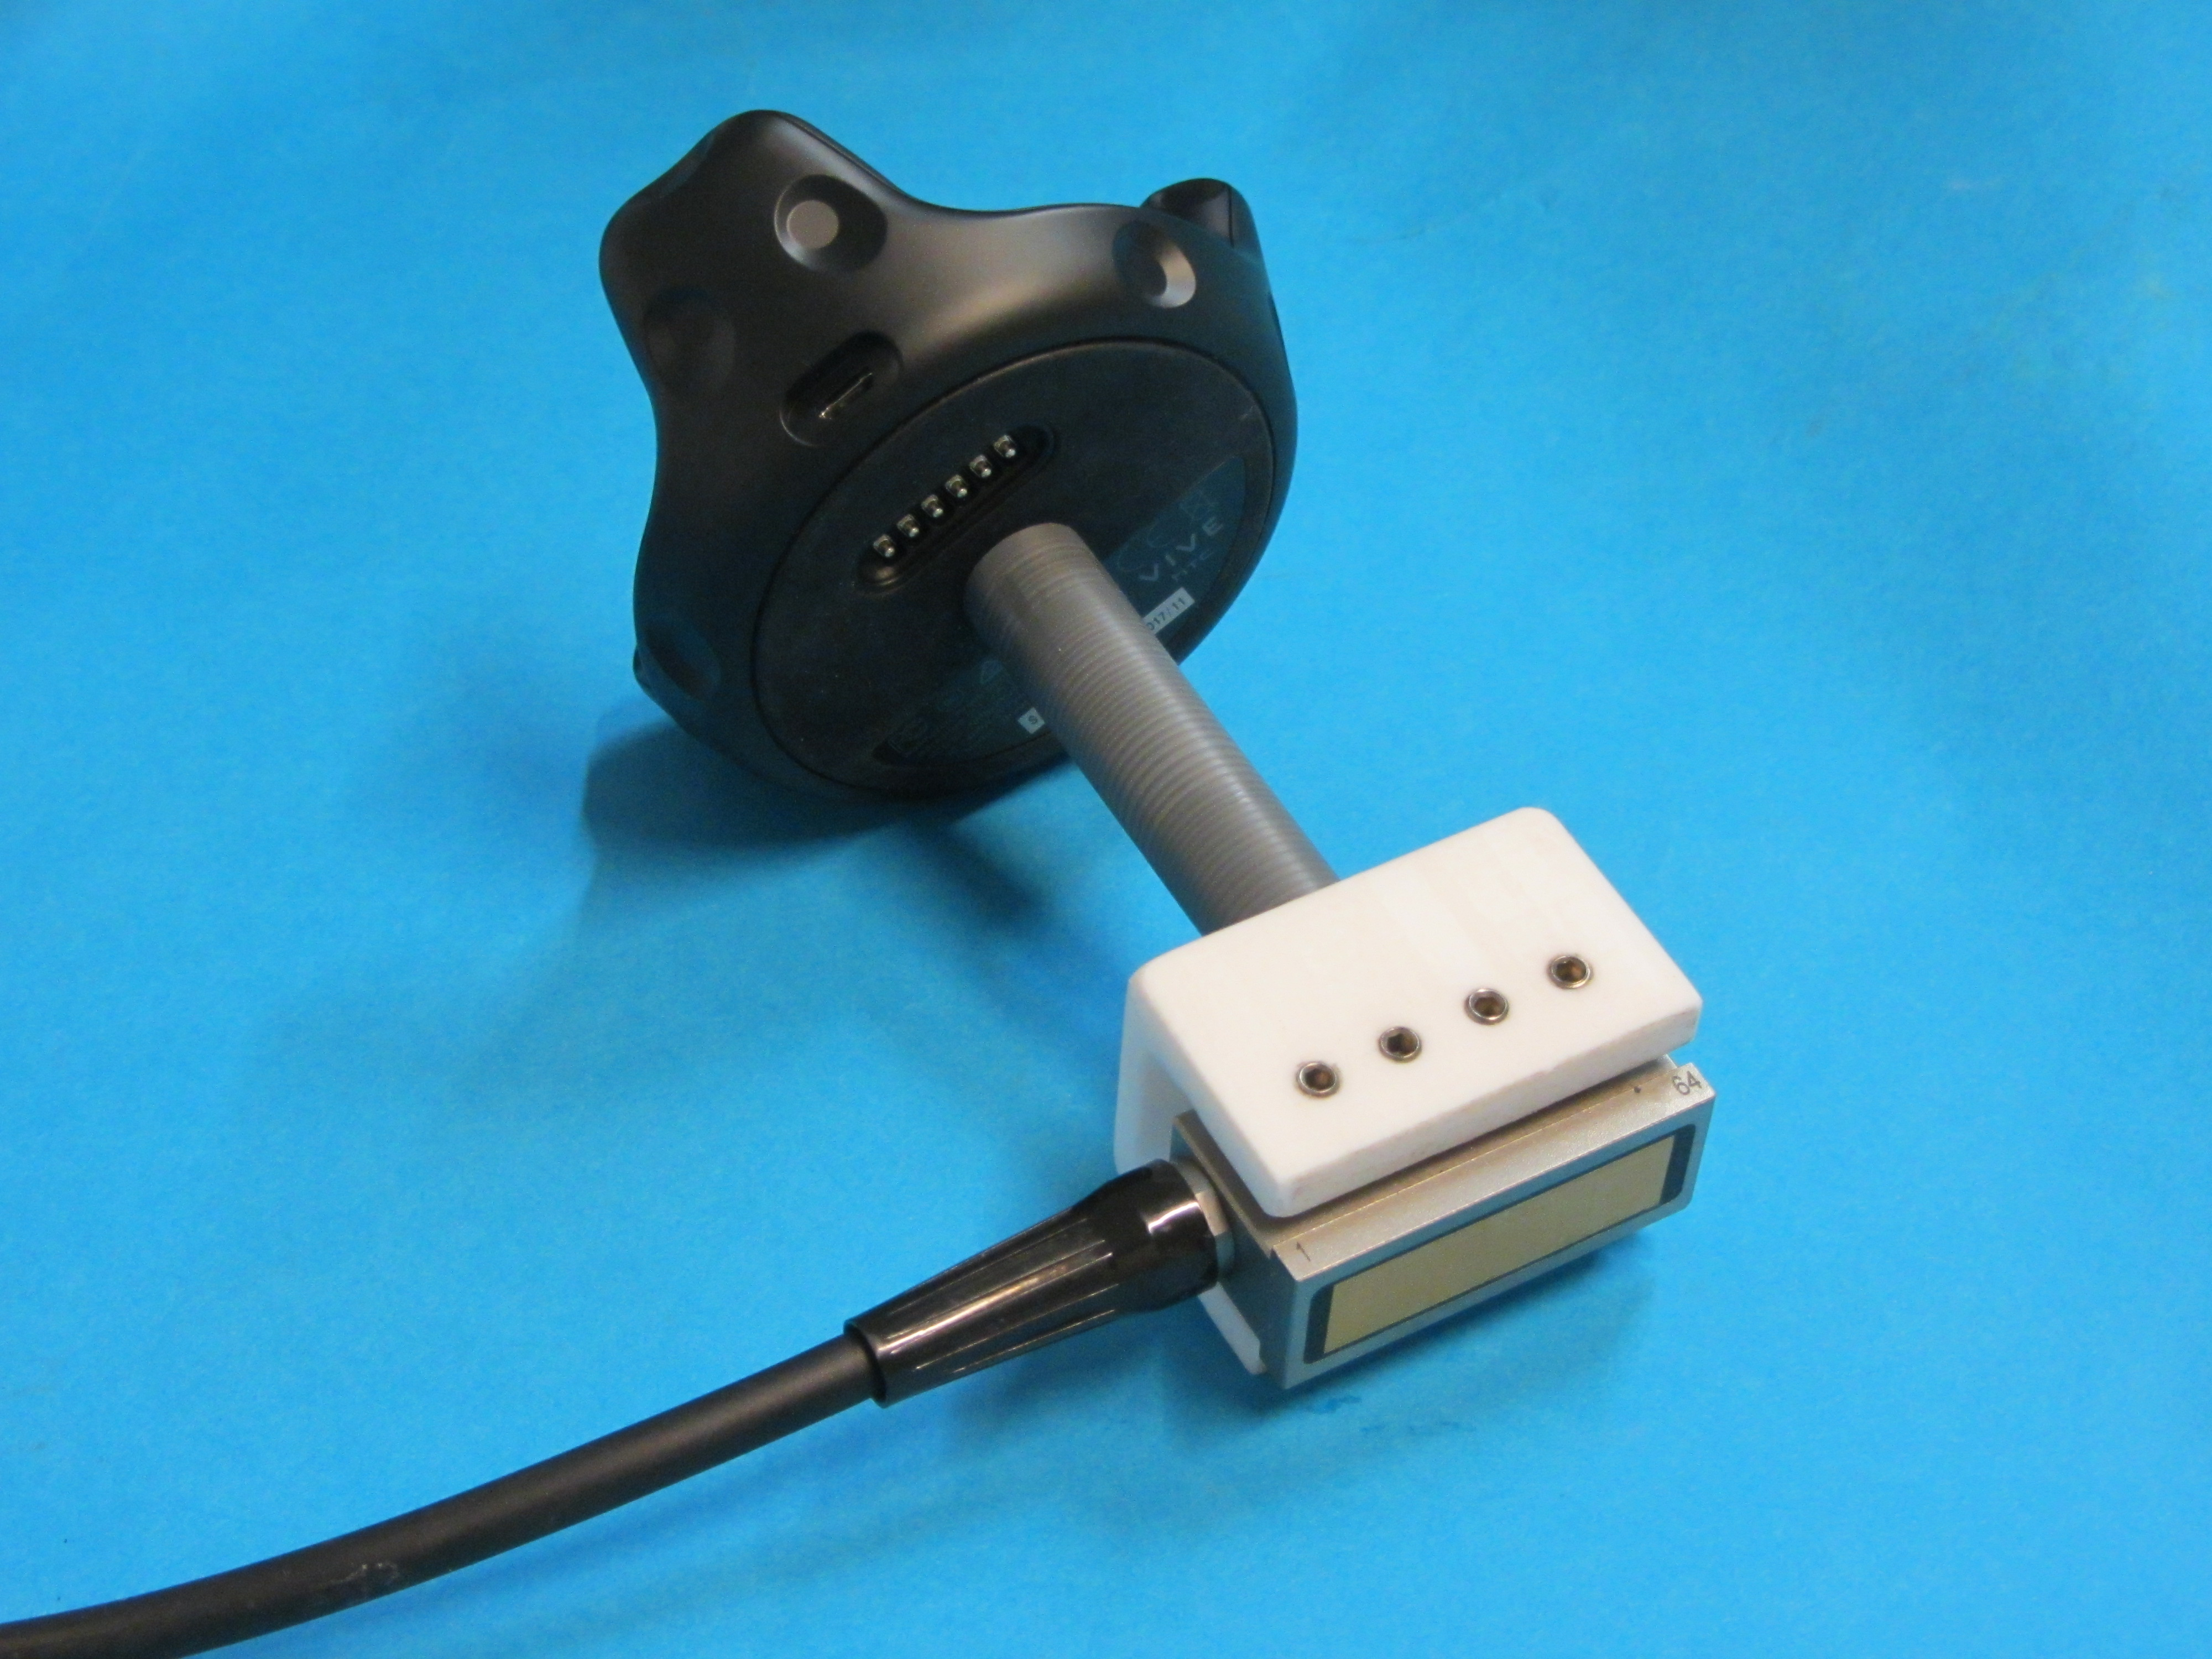
\includegraphics[width=79mm]{images/probemount.jpg}
        \caption{\label{fig:probemount} Probemount, that fixes \textit{VIVE--}Tracker to ultrasonic probe.}
    \end{center}
\end{figure}

\subsection{Detection of the coordinate system in worldspace}
The coordinate system of the surface to be measured is detected in two steps:
first a point--cloud of the surface is created by moving the tracked probe across it.
In the next step the parameters of the selected geometry in worldspace are calculated from this point--cloud using the Downhill--Simplex optimization by Nelder and Mead.
In a second step the used coordinate system is picked by placing the tracked probe at the desired origin and pressing the setup button.
As the specimen--geometry is already defined, only one more axis is required to define the orthogonal coordinate system.
this is done by placing the tracked probe on the X--Axis and pressing the setup button.

\subsection{Visualization of the tracking--data}
\label{sec:DrawVsErase}
To visualize the already traced path, a visual feedback is given to the inspector.
The feedback can be implemented in multiple ways, depending on the application.
The Path can either be drawn on the surface (DRAW), erased from a pre--colored area (ERASE), or be drawn onto a pre--colored area (HYBRID) (figure~\ref{fig:DrawVsErase}).

\begin{figure}[h!]
    \begin{center}
        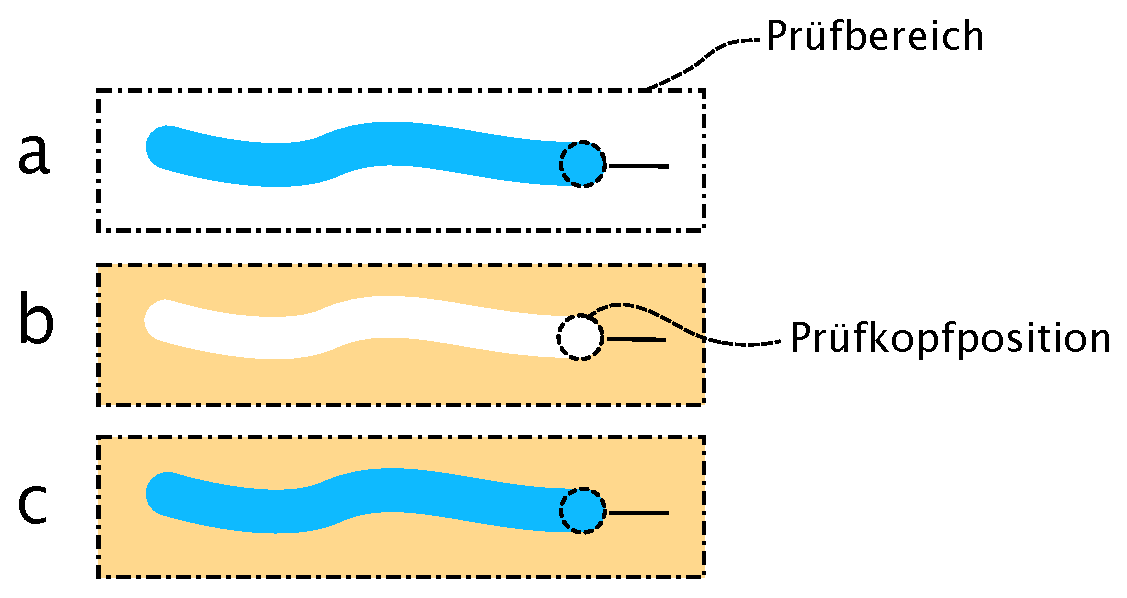
\includegraphics[width=79mm]{images/DrawVsErase.eps}
        \caption{\label{fig:DrawVsErase} Different methods to mark covered area.}
    \end{center}
\end{figure}

The main purpose of this visualization is to show possible gaps in the inspection, or to follow a predefined inspection--path.
In the case of SZMF, there is no specific inspection--plan that can give a pattern to erase, therefore DRAW was implemented.

\subsection{Continuous and singular logging of position}
The application allows the continuous logging of the probes position.
This protocol can be useful for documenting exactly which path was taken, and where exactly the imperfections were detected.
In addition to that, it is possible to log singular spots and store them for later use.

\section{Evaluation of the \textit{VIVE}--tracker accuracy}
The accuracy of the \textit{VIVE}--Tracker was determined in a experiment using an automated X--Y--scanner.
Both \textit{VIVE}--Basestations were positioned on opposite corners of the scanner, though one at a greater distance (figure~\ref{fig:precisionMeasurementSetup}).

\begin{figure}[h!]
    \begin{center}
        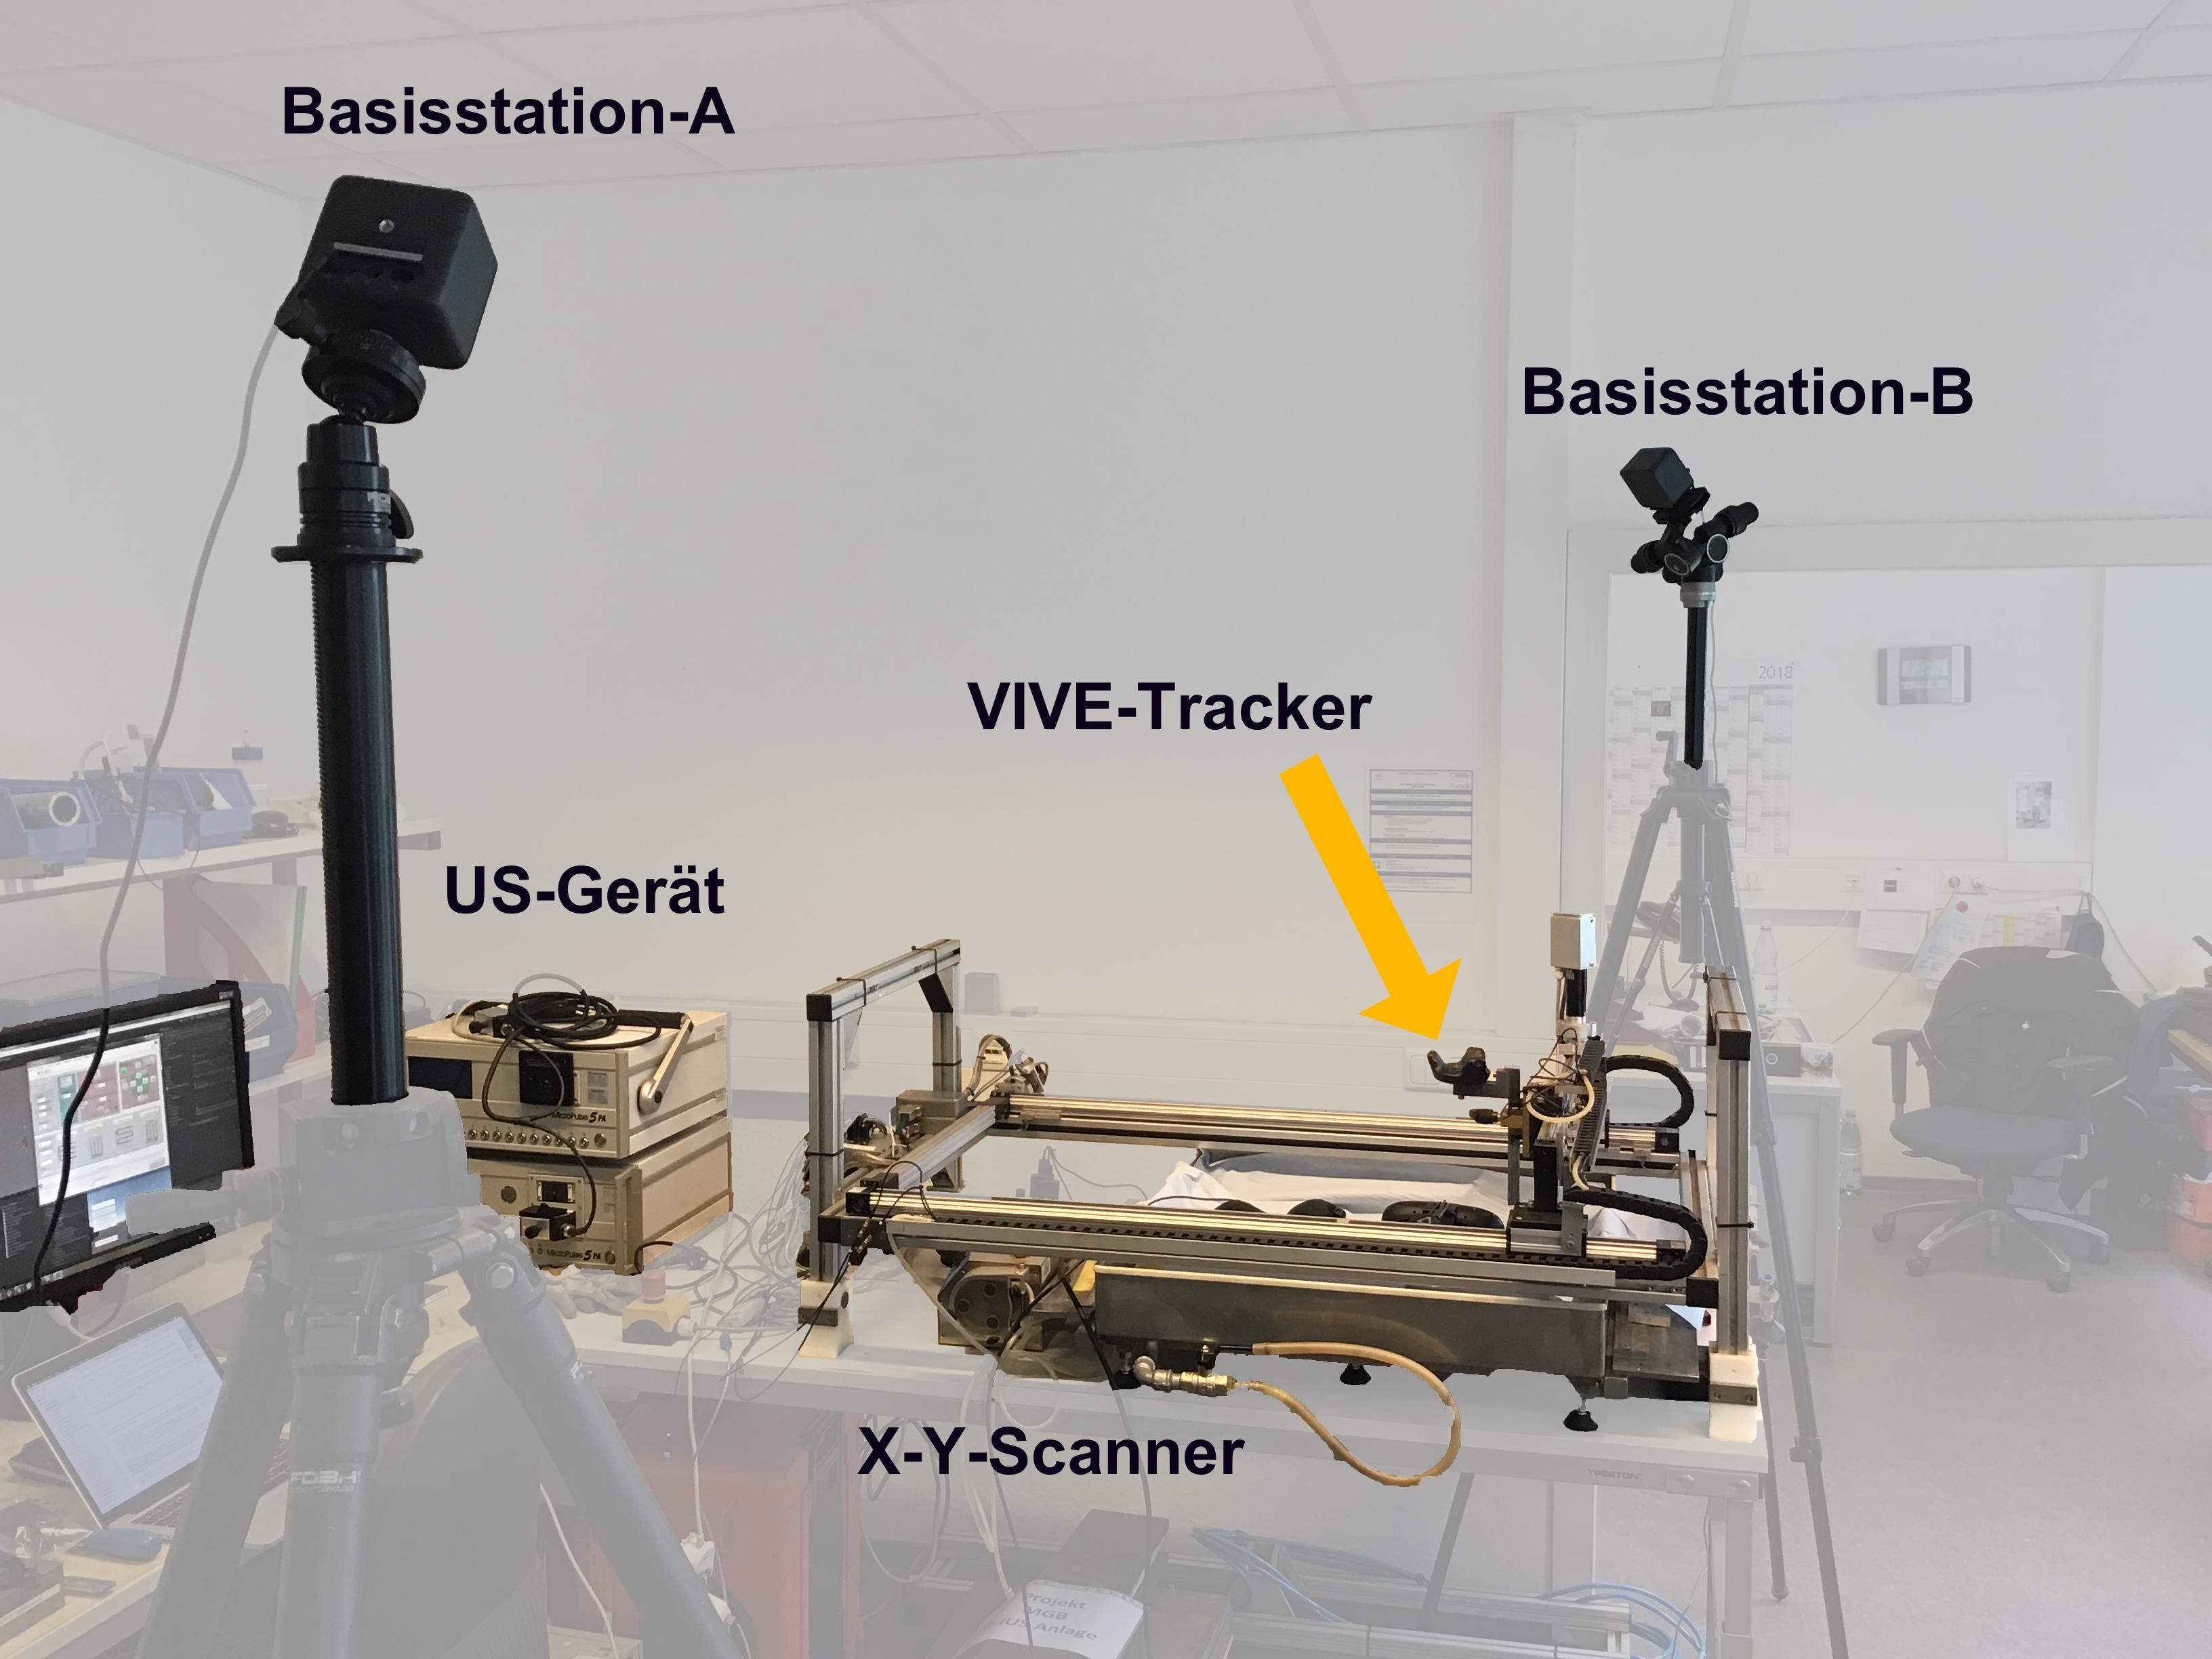
\includegraphics[width=79mm]{images/PrecisionMeasurement.jpg}
        \caption{\label{fig:precisionMeasurementSetup} Setup for the evaluation of the \textit{VIVE}--Precision. \textcolor{red}{Grafik muss noch übersetzt werden.}}
    \end{center}
\end{figure}

The tracker was screwed to the moving head of the scanner and moved in a comb structure over a surface of 400\,mm x 800\,mm.
During the process, the position of the tracker and absolute time was continuously logged.
In the beginning and end of each comb tine the movement was paused by 2\,s to identify the position in the log--file.\\

The evaluation was done by choosing the start position as a reference and calculating the difference between the distance of the measured and the calculated position to it.
These differences are plottet subject to the tine and type of comb.

\begin{figure}[h!]
    \begin{center}
        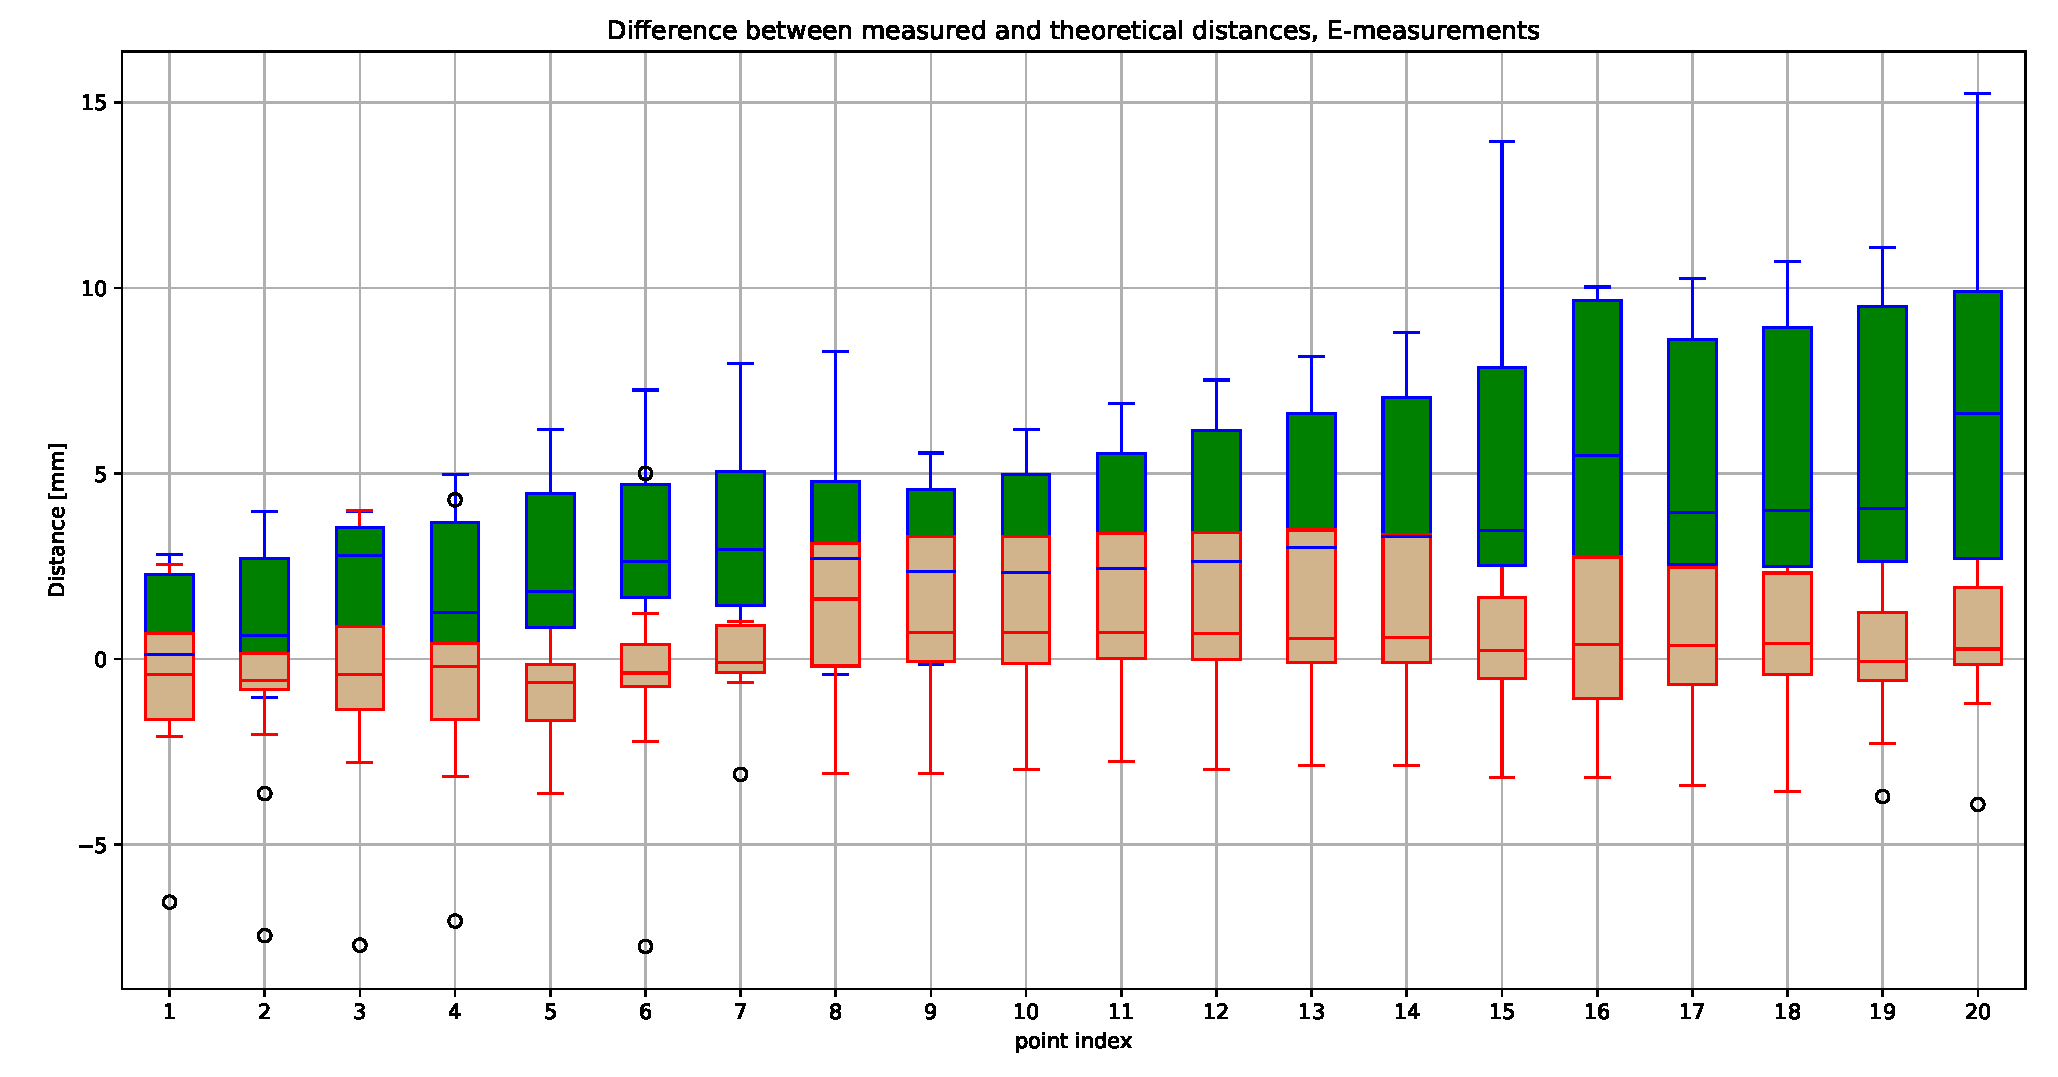
\includegraphics[width=79mm]{images/distancesBoxplot-E.eps}
        \caption{\label{fig:boxplotE} Difference between measured and theoretical distances to the reference point at the E--Positions.}
    \end{center}
\end{figure}

\begin{figure}[h!]
    \begin{center}
        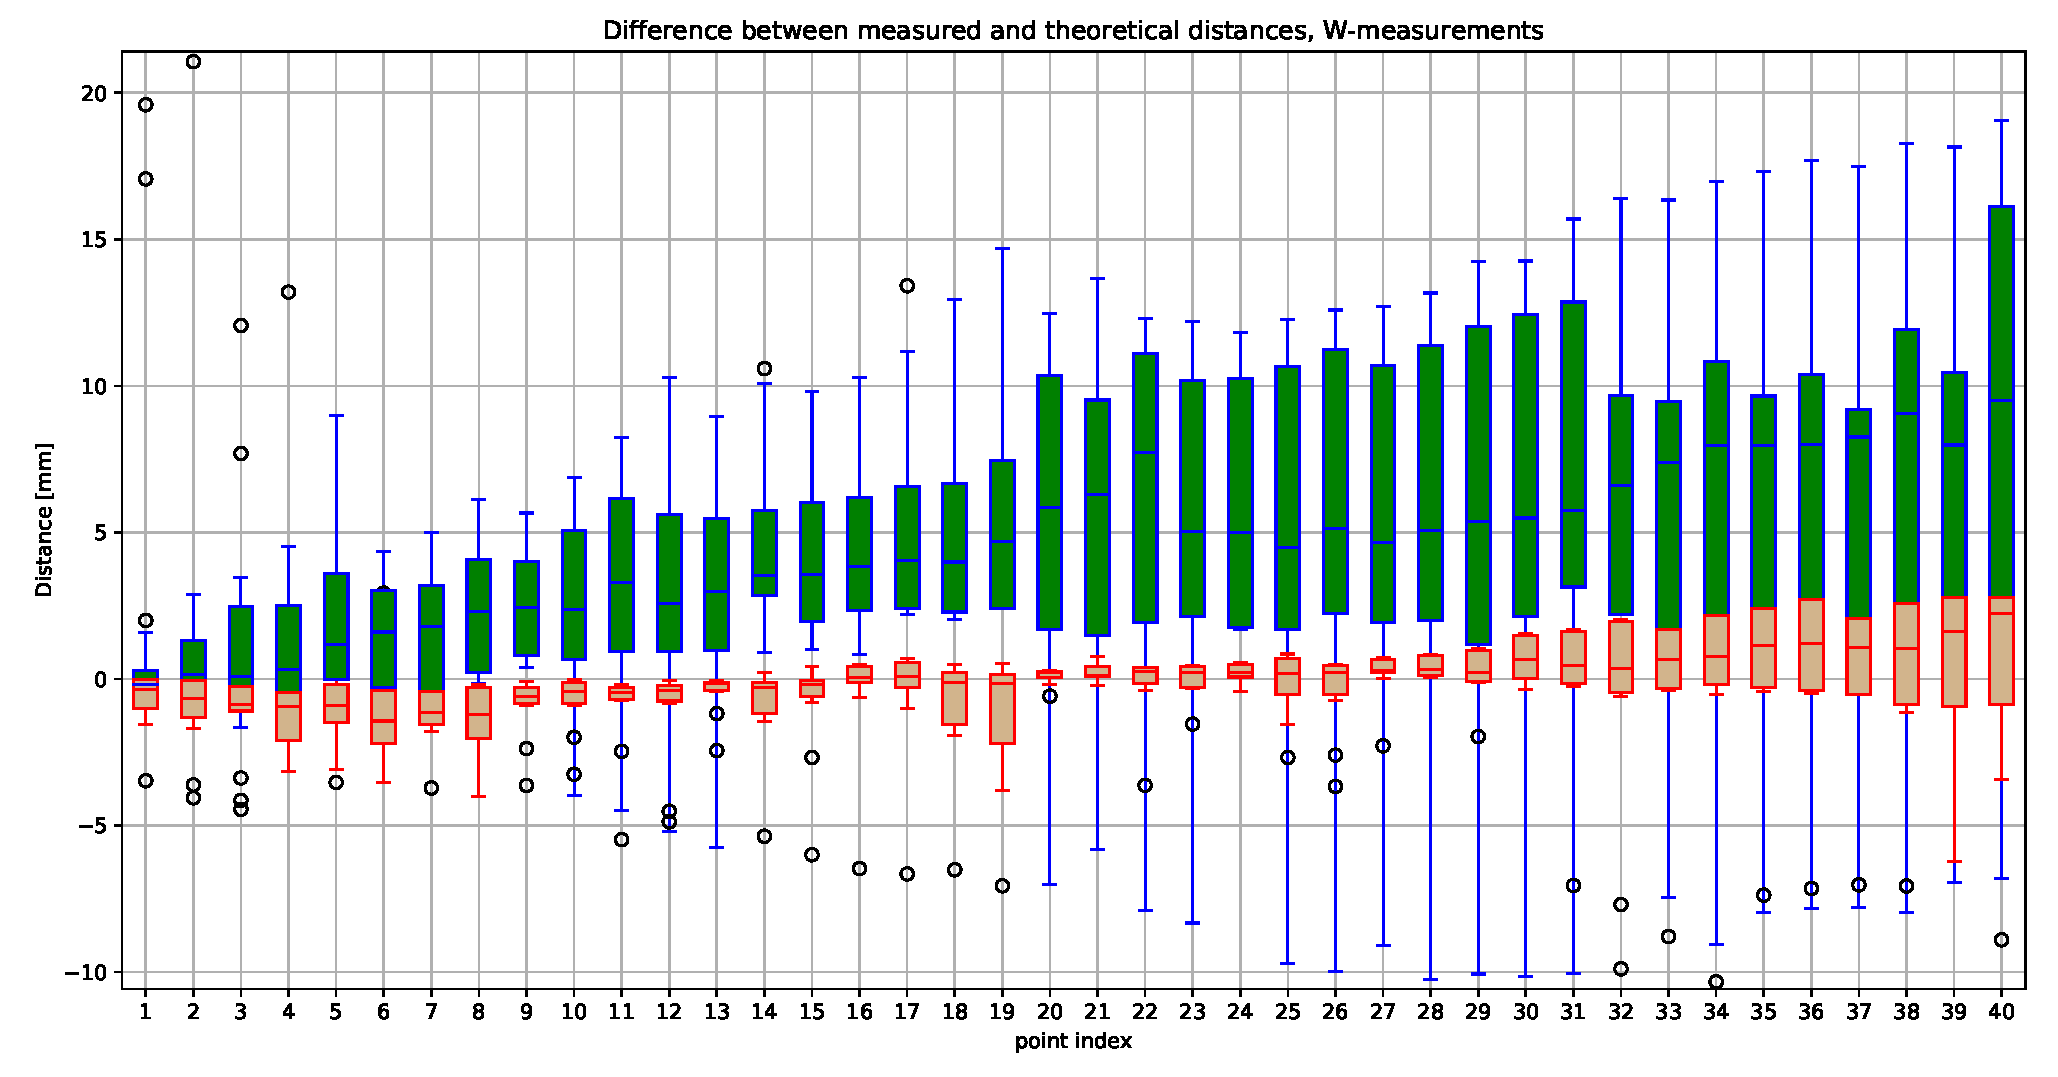
\includegraphics[width=79mm]{images/distancesBoxplot-W.eps}
        \caption{\label{fig:boxplotW} Difference between measured and theoretical distances to the reference point at the W--Positions.}
    \end{center}
\end{figure}

The results show a decline in quality as the surveypoints get closer to the closer basestation (basestation--B in figure~\ref{fig:precisionMeasurementSetup}) with an error up to 18\,mm.
In the opposite corner the values had a quality of about 1--2\,mm.
This can be explained by the rapidly declining quality as the proximity to the basestation is too small.

\section{Conclusion}

\begin{figure}[h!]
    \begin{center}
        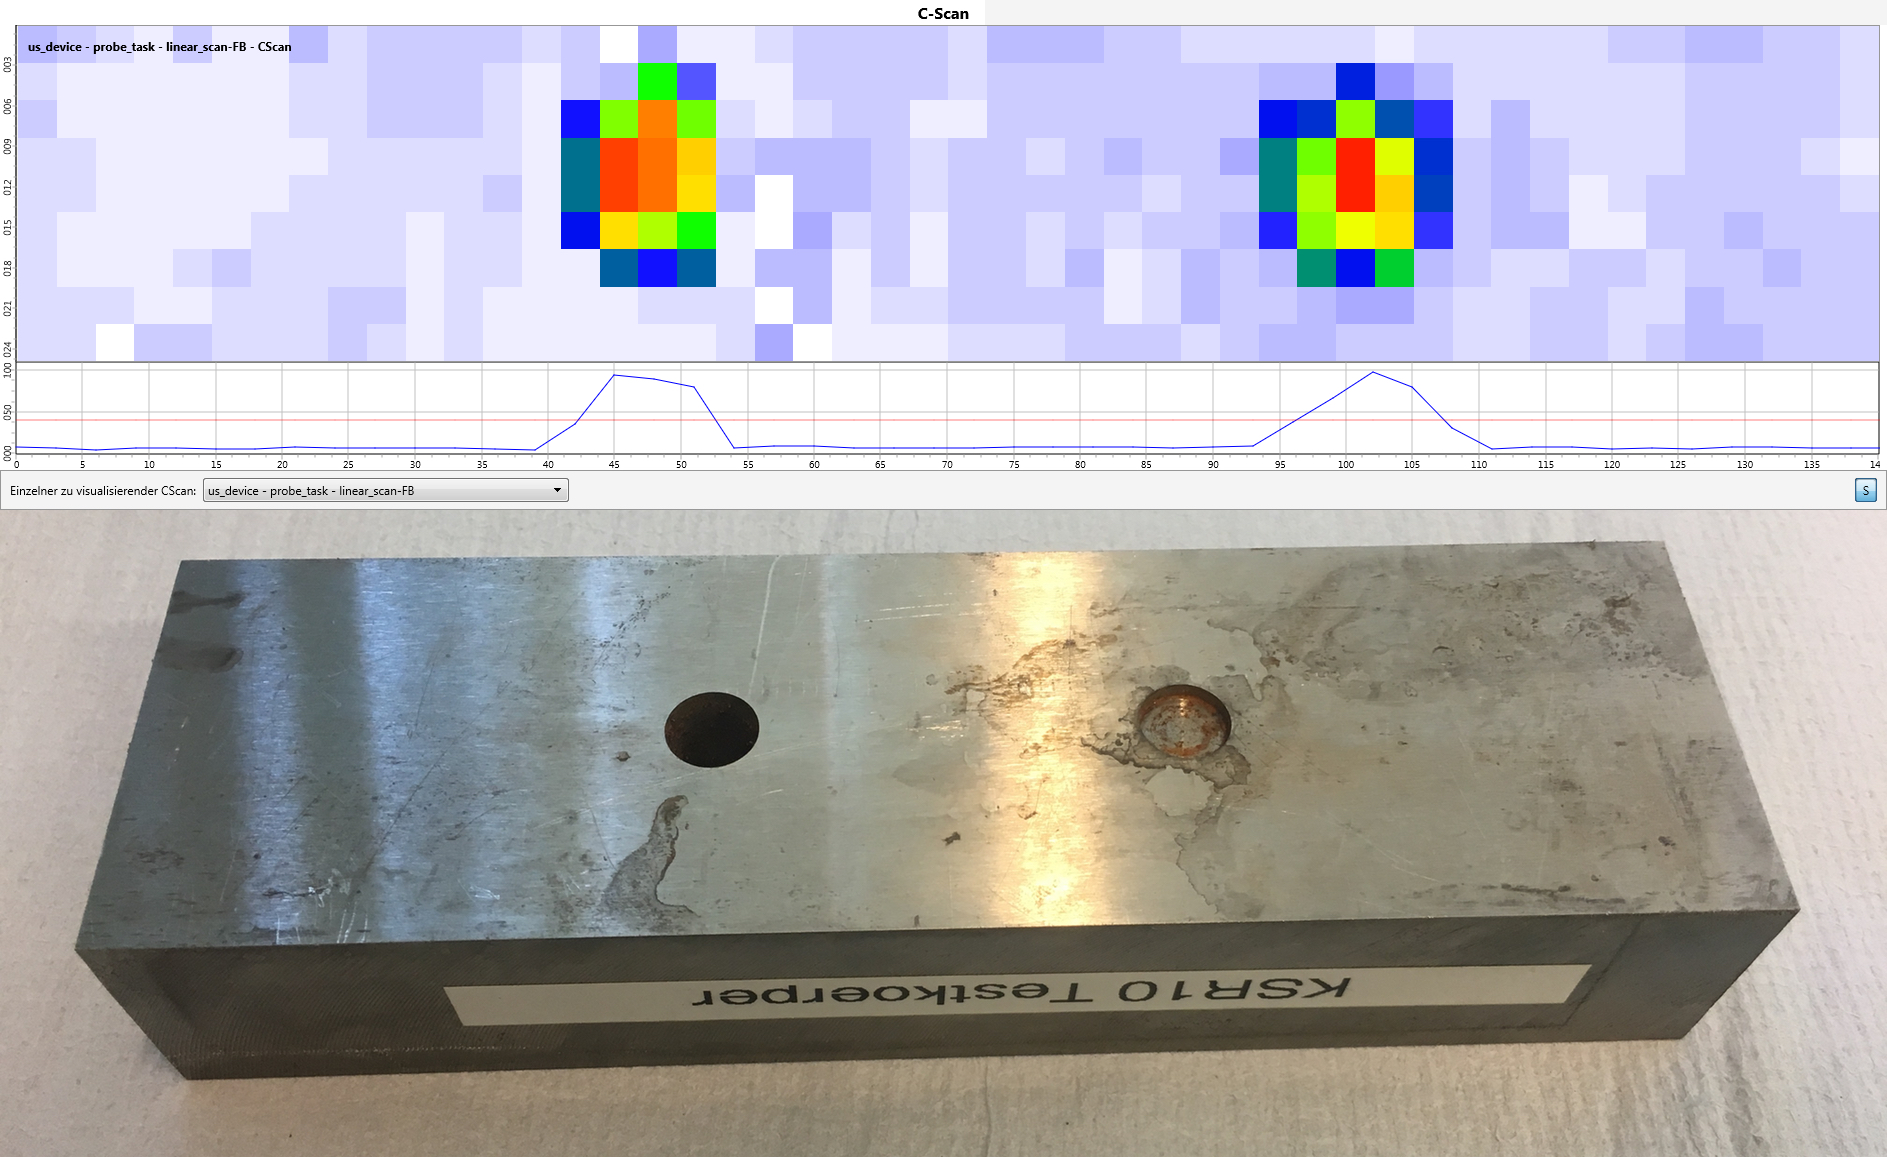
\includegraphics[width=79mm]{images/CScanARUS.jpg}
        \caption{\label{fig:resultCScan} C-Scan generated with the \textit{VIVE}--tracking system}
    \end{center}
\end{figure}

\VRARsetbibstyle
\bibliography{bibliography}

\end{document}
